\subsection{Reward Pools}
\label{subsec:reward_pools}

This section introduces the three reward pools: the \glsfirst{OP}, the \glsfirst{SP}, and the \glsfirst{PGP}. See \Cref{fig:network-rewards} for an illustration.

    {
        \begin{figure}[tb!]
            \centering
            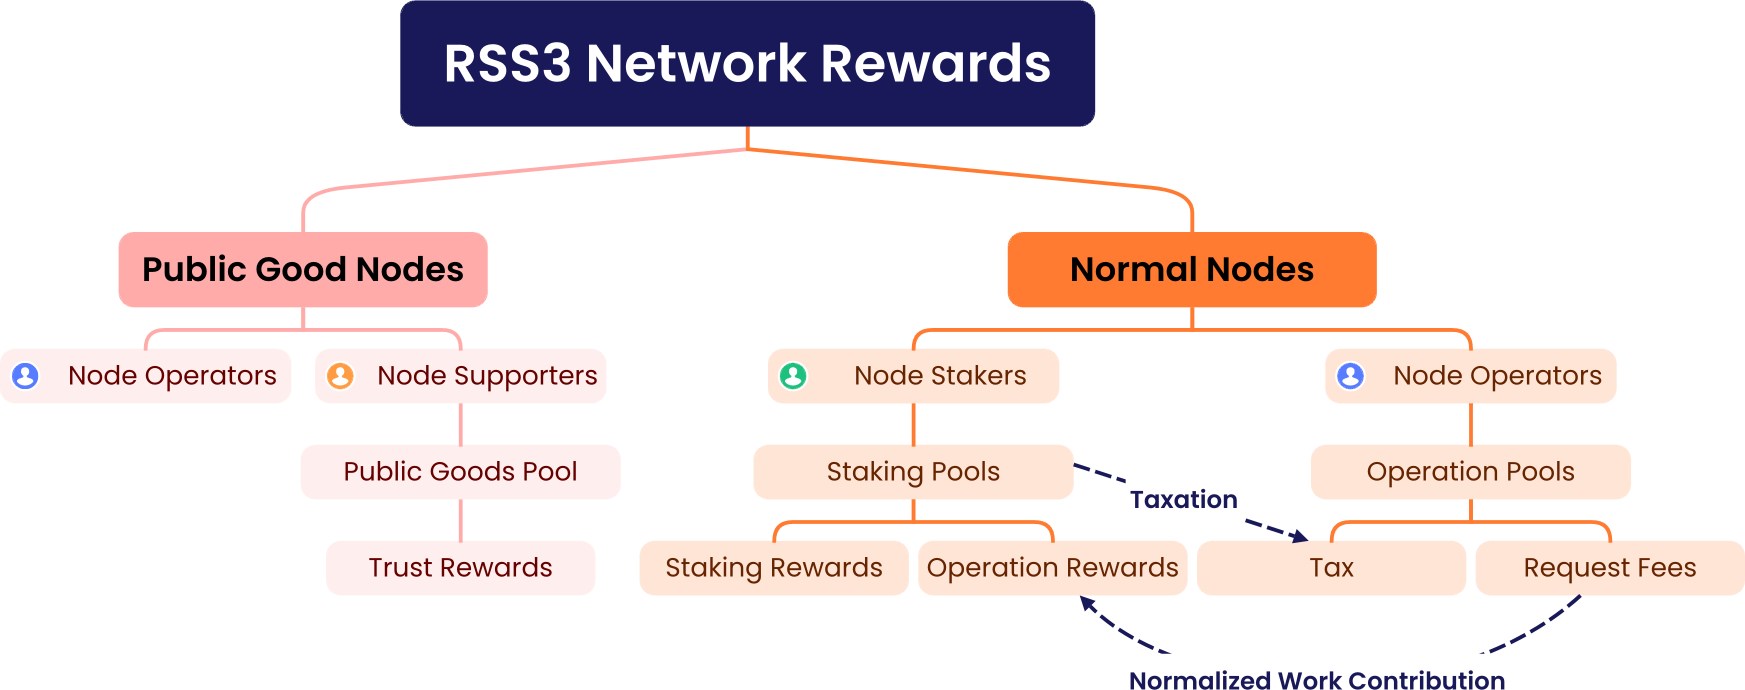
\includegraphics[width=\columnwidth]{figures/network-rewards.png}
            \caption{RSS3 \glsfmtlong{NR} distribution.
                The \glsfmtlong{NR} are allocated differently to Normal Nodes and Public Good Nodes.
                See \Cref{subsec:reward_pools} for details.}
            \label{fig:network-rewards}
        \end{figure}
    }

\subsubsection{\glsfmtlong{OP} (\operationPool)}
\label{subsubsec:operation_pool}

An \glsfirst{OP} is used to store tokens that are allocated to a Normal Node from two sources:
\begin{enumerate}
    \item The \gls{Fee} collected from requests served on the \gls{DSL}
    \item The \gls{Tax} collected from the Node's \stakingPool
\end{enumerate}

The \glsfmtlong{NO} can set a tax rate, \taxRate, which is applied to its \stakingPool.
The tax applies to the \glsfmtlong{NR} allocated to the Node's \stakingPool, not the staked tokens. See \Cref{subsubsec:taxation}.

Only the corresponding \glsfmtlong{NO} can withdraw tokens from its \operationPool, and the withdrawal is subject to a waiting period imposed by the Network.

\subsubsection{\glsfmtlong{SP} (\stakingPool)}
\label{subsubsec:staking_pool}

A \glsfirst{SP} is used to store staked tokens for a Normal Node. Network participants can stake tokens into a Normal Node's \stakingPool\ to increase the Node's chance to receive requests on the \gls{DSL}.

The allocation of \glsfmtlong{NR} into a Node's \stakingPool\ at the end of each epoch \epoch, is determined by two factors:
\begin{enumerate}
    \item \gls{OR}, the Node's normalized work contribution \work\ in proportion to the total work done on the \gls{DSL} (See \Cref{subsubsec:staking_rewards})
    \item \gls{SR}, the Node's \stakingPool\ size in proportion to the total staked tokens on the \gls{VSL} (See \Cref{subsubsec:operation_rewards})
\end{enumerate}

A tax \tax\ is then applied to the received Rewards, with the rate set by its \glsfmtlong{NO}.

\subsubsection{\glsfmtlong{PGP} (\publicGoodPool)}

A \glsfirst{PGP} is a unique reward pool that is shared by all Public Good Nodes.

As Public Good Nodes do not have their own \stakingPool, network participants entrust their tokens to the \publicGoodPool\ and signify their support to a designated Public Good Node.
